% =====================================================================
\chapter{Tinjauan Pustaka}
\label{bab:2}
% =====================================================================
Bab ini membahas penelitian terkait dan dasar teori yang digunakan dalam penelitian, meliputi sistem E-Office dan SOP layanan akademik, chatbot dan asisten virtual, \textit{Large Language Model}, \textit{Retrieval-Augmented Generation}, GraphRAG, pemodelan proses bisnis, \wgr{}, teknologi yang digunakan, serta metode evaluasi.

% ---------------------------------------------------------------------
\section{Penelitian Terkait}
\label{sec:terkait}
Penelitian terkait yang menjadi acuan dalam skripsi ini ditunjukkan pada Tabel~\ref{tab:terkait}. Penelitian-penelitian tersebut dikelompokkan berdasarkan objek studi dan pendekatan yang digunakan.

\begin{table}[htbp]
\caption{Penelitian Terkait}
\label{tab:terkait}
\centering\tabsetup
\begin{tabularx}{\linewidth}{|C{0.6cm}|L{3.0cm}|Y|L{3.6cm}|}
\hline\hdr
\hrow\textbf{No} & \textbf{Peneliti} & \textbf{Pendekatan dan Hasil} & \textbf{Keterbatasan} \\\hline
1 & \textcite{sutantio2026perbandingan} & Membandingkan RASA dan RAG pada chatbot layanan kemahasiswaan FSM dengan 7 SOP yang sama. Akurasi keduanya tidak berbeda signifikan, RASA jauh lebih cepat, sedangkan RAG lebih mudah disiapkan. & SOP diperlakukan sebagai teks; urutan langkah dan aktor tidak diukur. \\\hline
2 & \textcite{sahnah2026pengembangan} & Chatbot hibrida NLU-RASA dan LLM-RAG berbasis web (Next.js dan FastAPI) dengan metodologi ICONIX, diuji oleh responden mahasiswa. & Fokus pada rekayasa perangkat lunak; tidak ada evaluasi prosedural. \\\hline
3 & \textcite{lewis2020rag} & Memperkenalkan RAG yang menggabungkan \textit{retriever} padat dengan generator sekuens. & Konteks berupa teks tidak terstruktur. \\\hline
4 & \textcite{edge2024graphrag}; \textcite{guo2024lightrag} & GraphRAG dan LightRAG membangun graf entitas-relasi dengan LLM untuk pertanyaan global dan lokal. & Tidak menyimpan urutan eksekusi langkah. \\\hline
5 & \textcite{lin2026soprag} & SOPRAG menggunakan pakar graf alur dan graf entitas untuk menemukan SOP industri. & Indeks dipelajari pada skala besar; efek pemilihan dan penstrukturan tidak dipisahkan. \\\hline
6 & \textcite{wiratama2026procedure} & \wgr{} pada 7 SOP FSM dengan LLM lokal; KFR 0,955 dan cakupan langkah 1,000; pemilihan SOP menjadi faktor utama. & Masih berupa eksperimen; belum diterapkan pada sistem layanan. \\\hline
\end{tabularx}
\end{table}

Berdasarkan Tabel~\ref{tab:terkait}, penelitian di FSM telah menerapkan chatbot untuk SOP layanan kemahasiswaan, tetapi belum memodelkan urutan langkah dan aktor secara eksplisit. Sebaliknya, penelitian pendahuluan penulis telah menguji representasi alur kerja tersebut, tetapi belum menerapkannya sebagai layanan. Skripsi ini mengisi celah tersebut dengan menerapkan \wgr{} sebagai mesin asisten virtual pada sistem E-Office.

% ---------------------------------------------------------------------
\section{Sistem E-Office dan SOP Layanan Akademik}
\label{sec:eoffice}
Subbab ini membahas sistem persuratan digital E-Office yang menjadi tempat penerapan asisten virtual, serta struktur dokumen SOP yang menjadi basis pengetahuannya.

\subsection{Sistem Persuratan Digital E-Office}
E-Office adalah sistem informasi yang mendigitalkan proses perkantoran, terutama pembuatan, verifikasi, penandatanganan, dan pengarsipan surat. Di Indonesia, penerapan sistem semacam ini merupakan bagian dari Sistem Pemerintahan Berbasis Elektronik (SPBE) yang mendorong layanan administrasi terpadu berbasis elektronik \parencite{perpres95_2018}. Pada lingkungan akademik, E-Office memungkinkan mahasiswa mengajukan surat secara daring dan memantau prosesnya tanpa harus datang ke loket.

Sistem E-Office yang dikembangkan penulis memodelkan setiap surat sebagai entitas yang berpindah status secara berurutan. Alur status surat dan aktor yang memprosesnya ditunjukkan pada Gambar~\ref{fig:eoffice-status}. Mahasiswa mengajukan surat (\code{SUBMITTED}), surat diverifikasi oleh SA (\code{VERIFIED}), ditandatangani oleh MTU (\code{SIGNED}), lalu dicatat dan diberi nomor oleh UPA (\code{REGISTERED}). % TODO: tulis kepanjangan SA, MTU, dan UPA
Alur ini juga merupakan alur kerja berarah, sehingga cocok dengan pendekatan graf alur kerja yang digunakan untuk SOP.

\begin{figure}[htbp]
\centering
\begin{tikzpicture}[font=\normalsize,
  st/.style={draw, rounded corners=3pt, minimum width=2.6cm, minimum height=1cm, align=center, fill=g8},
  ac/.style={font=\normalsize\itshape, align=center},
  arr/.style={-{Stealth[length=2.2mm]}, thick}]
\node[st] (s1) at (0,0)    {\code{SUBMITTED}};
\node[st] (s2) at (3.6,0)  {\code{VERIFIED}};
\node[st] (s3) at (7.2,0)  {\code{SIGNED}};
\node[st] (s4) at (10.8,0) {\code{REGISTERED}};
\draw[arr] (s1) -- (s2); \draw[arr] (s2) -- (s3); \draw[arr] (s3) -- (s4);
\node[ac, below=0.35cm of s1] {Mahasiswa\\mengajukan};
\node[ac, below=0.35cm of s2] {SA\\memverifikasi};
\node[ac, below=0.35cm of s3] {MTU\\menandatangani};
\node[ac, below=0.35cm of s4] {UPA\\mencatat};
\end{tikzpicture}
\caption{Alur Status Surat pada Sistem E-Office}
\label{fig:eoffice-status}
\end{figure}

\subsection{Standar Operasional Prosedur Layanan Akademik}
\label{sec:sop}
Standar Operasional Prosedur (SOP) adalah dokumen yang menetapkan langkah-langkah baku untuk menyelesaikan suatu layanan. FSM Universitas Diponegoro menerbitkan 7 SOP layanan mahasiswa yang masing-masing terdiri atas satu halaman berbahasa Indonesia dengan total 44 langkah bernomor \parencite{wiratama2026procedure}. Seluruh SOP berbentuk urutan linier tanpa percabangan. Struktur dokumen SOP ditunjukkan pada Gambar~\ref{fig:anatomi-sop}: judul, kalimat tujuan yang dapat memuat batas waktu pemrosesan, serta langkah bernomor yang subjek kalimatnya adalah pelaksana langkah, dan dapat diikuti baris \textit{Waktu}, \textit{Dokumen yang dibutuhkan}, dan \textit{Output}.

\begin{figure}[htbp]
\centering
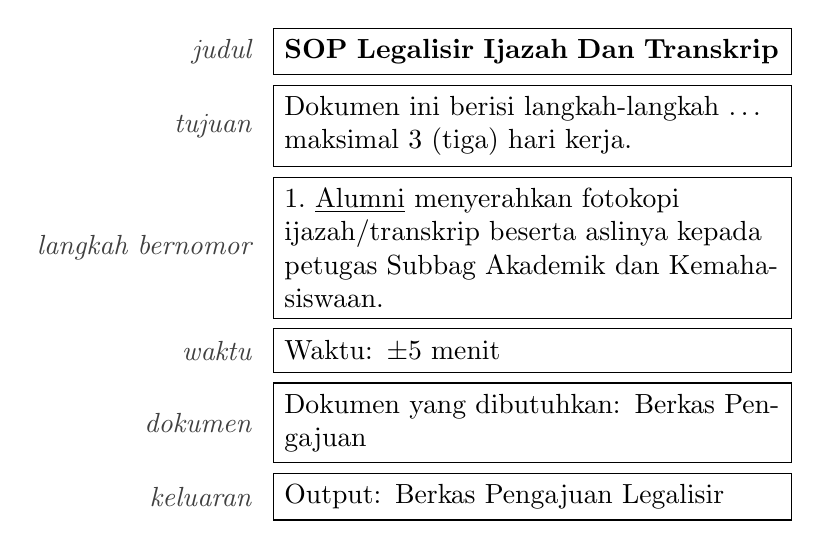
\begin{tikzpicture}[font=\normalsize,
  doc/.style={draw, fill=white, align=left, inner sep=1.4mm, text width=6.3cm},
  tag/.style={font=\normalsize\itshape, anchor=east, text=black!75}]
\node[doc] (title) at (0,0) {\textbf{SOP Legalisir Ijazah Dan Transkrip}};
\node[doc, anchor=north] (purp) at ([yshift=-1.2mm]title.south) {Dokumen ini berisi langkah-langkah \dots\ maksimal 3 (tiga) hari kerja.};
\node[doc, anchor=north] (step) at ([yshift=-1.2mm]purp.south) {1.\ \underline{Alumni} menyerahkan fotokopi ijazah/transkrip beserta aslinya kepada petugas Subbag Akademik dan Kemahasiswaan.};
\node[doc, anchor=north] (wkt) at ([yshift=-1.2mm]step.south) {Waktu: $\pm$5 menit};
\node[doc, anchor=north] (dok) at ([yshift=-1.2mm]wkt.south) {Dokumen yang dibutuhkan: Berkas Pengajuan};
\node[doc, anchor=north] (out) at ([yshift=-1.2mm]dok.south) {Output: Berkas Pengajuan Legalisir};
\node[tag] at ([xshift=-1.5mm]title.west) {judul};
\node[tag] at ([xshift=-1.5mm]purp.west) {tujuan};
\node[tag] at ([xshift=-1.5mm]step.west) {langkah bernomor};
\node[tag] at ([xshift=-1.5mm]wkt.west) {waktu};
\node[tag] at ([xshift=-1.5mm]dok.west) {dokumen};
\node[tag] at ([xshift=-1.5mm]out.west) {keluaran};
\end{tikzpicture}
\caption{Struktur Dokumen SOP FSM (Contoh Langkah 1 SOP Legalisir)}
\label{fig:anatomi-sop}
\end{figure}

Langkah-langkah SOP dilaksanakan oleh 15 peran organisasi, mulai dari mahasiswa, program studi, pimpinan fakultas, unit administrasi fakultas, hingga tingkat universitas. Mahasiswa melaksanakan 21 dari 44 langkah, dan beberapa peran fakultas terlibat di lebih dari satu SOP \parencite{wiratama2026procedure}. Akibatnya, SOP yang berbeda berbagi aktor dan kosakata yang sama, yang menyulitkan temu kembali berbasis kemiripan teks.

% ---------------------------------------------------------------------
\section{Chatbot dan Asisten Virtual}
\label{sec:chatbot}
Chatbot adalah program yang berinteraksi dengan pengguna melalui bahasa alami \parencite{adamopoulou2020overview}. Chatbot awal seperti ELIZA bekerja dengan pencocokan pola \parencite{weizenbaum1966eliza}, kemudian berkembang menjadi chatbot berbasis \textit{Natural Language Understanding} (NLU) yang mengklasifikasikan maksud (\textit{intent}) dan mengekstraksi entitas, seperti RASA. Asisten virtual generasi terbaru menggunakan LLM sehingga dapat menyusun jawaban baru tanpa harus menyiapkan seluruh pola percakapan terlebih dahulu \parencite{jurafsky2026slp}. Kelemahannya, jawaban LLM perlu dikendalikan agar tetap sesuai dengan sumber resmi, yang menjadi alasan penggunaan RAG pada penelitian ini.

% ---------------------------------------------------------------------
\section{Large Language Model}
\label{sec:llm}
Subbab ini membahas arsitektur dasar LLM serta penggunaan LLM berukuran kecil yang dijalankan secara lokal.

\subsection{Arsitektur Transformer}
LLM modern dibangun di atas arsitektur Transformer yang menggunakan mekanisme \textit{self-attention} untuk menghitung hubungan antartoken dalam satu urutan \parencite{vaswani2017attention}. Perhitungan \textit{attention} ditunjukkan pada Persamaan~\ref{eq:attention}:
\begin{equation}
\mathrm{Attention}(Q,K,V)=\mathrm{softmax}\!\left(\frac{QK^{\top}}{\sqrt{d_k}}\right)V
\label{eq:attention}
\end{equation}
\begin{keterangan}
$Q$ & Matriks \textit{query} hasil proyeksi representasi token \\
$K$ & Matriks \textit{key} hasil proyeksi representasi token \\
$V$ & Matriks \textit{value} hasil proyeksi representasi token \\
$d_k$ & Dimensi vektor \textit{key} \\
\end{keterangan}

Model yang dilatih pada korpus teks berskala besar dengan tujuan memprediksi token berikutnya mampu mengerjakan berbagai tugas hanya dengan instruksi dan sedikit contoh di dalam \textit{prompt} \parencite{brown2020gpt3}. Kemampuan inilah yang memungkinkan LLM digunakan sebagai generator jawaban pada asisten virtual.

\subsection{LLM Lokal}
LLM berbobot terbuka seperti LLaMA \parencite{touvron2023llama} dan Gemma \parencite{gemmateam2024gemma} dapat dijalankan pada perangkat milik institusi. Ollama menyediakan layanan untuk mengunduh, menjalankan, dan memanggil model tersebut melalui antarmuka HTTP lokal \parencite{ollama2023}. Penggunaan LLM lokal menghindari biaya per kueri dan menjaga data tetap di dalam jaringan kampus. Akan tetapi, model berukuran kecil memiliki kapasitas penalaran terbatas dan lebih mudah terganggu ketika konteks memuat banyak informasi yang tidak relevan \parencite{liu2024lost}. LLM juga dapat berhalusinasi, yaitu menghasilkan informasi yang tidak didukung sumber \parencite{ji2023hallucination}. Oleh karena itu, konteks yang diberikan kepada model kecil perlu ringkas dan tepat sasaran.

% ---------------------------------------------------------------------
\section{Retrieval-Augmented Generation}
\label{sec:rag}
\textit{Retrieval-Augmented Generation} (RAG) adalah pendekatan yang mengondisikan generator pada dokumen hasil temu kembali \parencite{lewis2020rag,church2024emerging}. Alur umum RAG ditunjukkan pada Gambar~\ref{fig:rag}. Pada tahap luring, dokumen dipotong, diubah menjadi vektor, dan disimpan dalam basis data vektor. Pada tahap daring, pertanyaan diubah menjadi vektor, potongan yang paling mirip diambil, lalu disusun bersama pertanyaan menjadi \textit{prompt} untuk LLM \parencite{gao2023ragsurvey}.

\begin{figure}[htbp]
\centering
\begin{tikzpicture}[font=\normalsize,
  box/.style={draw, rounded corners=2pt, align=center, minimum height=1.1cm, text width=2.2cm, fill=white},
  arr/.style={-{Stealth[length=2mm]}, thick},
  lane/.style={draw=g60, rounded corners=4pt, fill=g6, inner sep=2.5mm}]
\node[box] (d) at (0,0) {Dokumen\\SOP};
\node[box] (c) at (3.2,0) {\textit{Chunking}};
\node[box] (e) at (6.4,0) {Embedding};
\node[box] (v) at (9.6,0) {Basis data\\vektor};
\draw[arr] (d)--(c); \draw[arr] (c)--(e); \draw[arr] (e)--(v);
\node[box] (q) at (0,-2.6) {Pertanyaan};
\node[box] (r) at (3.2,-2.6) {Temu kembali\\top-$k$};
\node[box] (p) at (6.4,-2.6) {\textit{Prompt}:\\konteks + tanya};
\node[box] (g) at (9.6,-2.6) {LLM\\(generator)};
\draw[arr] (q)--(r); \draw[arr] (r)--(p); \draw[arr] (p)--(g);
\draw[arr] (v.south) -- ++(0,-0.55) -| (r.north);
\begin{scope}[on background layer]
\node[lane, fit=(d)(v)] (off) {};
\node[lane, fit=(q)(g)] (on) {};
\end{scope}
\node[anchor=south west, font=\normalsize\bfseries] at (off.north west) {Tahap luring (sekali)};
\node[anchor=north west, font=\normalsize\bfseries] at (on.south west) {Tahap daring (setiap pertanyaan)};
\end{tikzpicture}
\caption{Alur Umum \textit{Retrieval-Augmented Generation}}
\label{fig:rag}
\end{figure}

\subsection{Chunking}
\textit{Chunking} adalah proses memecah dokumen menjadi potongan yang dapat dicari. Ukuran potongan menentukan keseimbangan antara kelengkapan konteks dan ketepatan temu kembali. Pada penelitian pendahuluan, dokumen dipotong dengan jendela 1.700 karakter dan tumpang tindih 100 karakter. Karena setiap SOP FSM lebih pendek dari 1.650 karakter, setiap SOP menjadi tepat satu potongan, sehingga pencarian tiga potongan teratas selalu memasukkan tiga SOP utuh ke dalam \textit{prompt} \parencite{wiratama2026procedure}.

\subsection{Embedding Teks}
\textit{Embedding} adalah representasi teks dalam bentuk vektor berdimensi tetap yang menempatkan teks bermakna serupa pada posisi yang berdekatan. Model \textit{embedding} kalimat seperti Sentence-BERT \parencite{reimers2019sbert} dan E5 \parencite{wang2022e5} dilatih secara kontrastif agar pasangan pertanyaan dan dokumen yang relevan memiliki kemiripan tinggi. Penelitian ini menggunakan \texttt{all-indo-e5-small-v4}, yaitu model E5 untuk bahasa Indonesia \parencite{lazarusnlp2024e5}.

\subsection{Basis Data Vektor dan Ukuran Kemiripan}
Basis data vektor menyimpan \textit{embedding} beserta metadata dan menyediakan pencarian tetangga terdekat. Chroma \parencite{chroma2023} digunakan pada tahap eksperimen, sedangkan pgvector \parencite{pgvector2021} memungkinkan pencarian vektor di dalam PostgreSQL yang juga digunakan oleh E-Office. Kemiripan antara vektor pertanyaan dan vektor dokumen dihitung dengan \textit{cosine similarity} seperti pada Persamaan~\ref{eq:cosine}:
\begin{equation}
\cos(\mathbf{q},\mathbf{d})=\frac{\mathbf{q}\cdot\mathbf{d}}{\lVert\mathbf{q}\rVert\,\lVert\mathbf{d}\rVert}
\label{eq:cosine}
\end{equation}
\begin{keterangan}
$\mathbf{q}$ & Vektor \textit{embedding} pertanyaan \\
$\mathbf{d}$ & Vektor \textit{embedding} potongan dokumen \\
$\lVert\cdot\rVert$ & Panjang (norma Euclidean) vektor \\
\end{keterangan}

\subsection{Varian RAG}
\label{sec:varian-rag}
Beberapa varian RAG yang digunakan sebagai pembanding dalam penelitian ini sebagai berikut:
\begin{enumerate}
\item Naive RAG, yang langsung memasukkan $k$ potongan teratas hasil temu kembali padat ke dalam \textit{prompt} \parencite{gao2023ragsurvey,karpukhin2020dpr}.
\item Hybrid RAG, yang menggabungkan temu kembali leksikal BM25 \parencite{robertson2009bm25} dengan temu kembali padat menggunakan \textit{reciprocal rank fusion} \parencite{cormack2009rrf}.
\item Agentic RAG, yang menyelingi penalaran dan pencarian secara bergantian seperti pada ReAct \parencite{yao2023react}.
\item Corrective RAG dan Self-RAG, yang menilai kualitas bukti dan menulis ulang kueri ketika bukti lemah \parencite{yan2024crag,asai2024selfrag}.
\end{enumerate}

Seluruh varian tersebut menyerahkan teks tidak terstruktur kepada generator, sehingga urutan langkah dan aktor pada setiap langkah hanya tersirat di dalam kalimat dan harus disimpulkan sendiri oleh LLM.

% ---------------------------------------------------------------------
\section{GraphRAG}
\label{sec:graphrag}
GraphRAG menambahkan relasi eksplisit antarbukti dalam bentuk graf \parencite{peng2024graphragsurvey,pan2024unifying}. Microsoft GraphRAG mengekstraksi entitas dan relasi menggunakan LLM, mengelompokkannya menjadi komunitas, lalu meringkas setiap komunitas \parencite{edge2024graphrag}. LightRAG mengindeks entitas dan relasi pada dua tingkat untuk pertanyaan lokal dan global \parencite{guo2024lightrag}, sedangkan HippoRAG menjalankan Personalized PageRank pada graf entitas \parencite{gutierrez2024hipporag}. Graf-graf tersebut menyimpan tripel entitas $(h,r,t)$ tanpa konsep urutan, percabangan, atau status eksekusi.

Penelitian yang lebih baru mulai memperhatikan urutan. SOPRAG menggunakan pakar graf alur dan graf entitas untuk menemukan SOP industri \parencite{lin2026soprag}, dan \textit{Order-Aware Hypergraph} RAG memodelkan transisi menggunakan \textit{hyperedge} \parencite{wu2026okhrag}. Perbandingan unit konteks yang diterima generator pada setiap kelompok metode ditunjukkan pada Tabel~\ref{tab:posisi}.

\begin{table}[htbp]
\caption{Perbandingan Unit Konteks yang Diterima Generator}
\label{tab:posisi}
\centering\tabsetup
\begin{tabularx}{\linewidth}{|C{0.6cm}|L{3.6cm}|Y|L{2.0cm}|L{2.0cm}|}
\hline\hdr
\hrow\textbf{No} & \textbf{Kelompok Metode} & \textbf{Unit Konteks} & \textbf{Urutan Langkah} & \textbf{Aktor per Langkah} \\\hline
1 & Naive, Hybrid, Agentic, Corrective RAG & Potongan teks tidak terstruktur & Tersirat & Tersirat \\\hline
2 & GraphRAG berbasis entitas & Tripel entitas-relasi dan teks & Tidak ada & Tripel relasi \\\hline
3 & \wgr{} & Blok alur kerja berarah dan potongan teks & Eksplisit & Eksplisit \\\hline
\end{tabularx}
\end{table}

% ---------------------------------------------------------------------
\section{Pemodelan Proses Bisnis dan Graf Alur Kerja}
\label{sec:bpm}
\textit{Business Process Management} (BPM) memodelkan prosedur sebagai alur kerja berarah yang terdiri atas aktivitas, peristiwa, dan aliran kendali \parencite{dumas2018fundamentals}. Notasi BPMN menambahkan \textit{swimlane} untuk aktor dan \textit{gateway} untuk percabangan \parencite{omg2011bpmn}, dan model proses dapat diekstraksi dari teks berbahasa alami \parencite{friedrich2011process}.

Secara formal, sebuah prosedur $p$ dapat dinyatakan sebagai graf berarah $G_p=(V_p,E_p)$ dengan $V_p$ himpunan simpul dan $E_p\subseteq V_p\times V_p$ himpunan sisi. Jika graf tidak memiliki siklus, simpul-simpulnya dapat diurutkan secara topologis sehingga setiap langkah selalu muncul setelah langkah prasyaratnya \parencite{kahn1962topological}. Sifat ini menjadi dasar metrik \textit{Topological Inversion Rate} yang dibahas pada Subbab~\ref{sec:metrik}. Dalam penelitian ini, graf alur kerja tidak digunakan untuk simulasi atau pemeriksaan kepatuhan, melainkan sebagai media temu kembali dan penyusunan \textit{prompt}.

% ---------------------------------------------------------------------
\section{Process-Aware Workflow GraphRAG}
\label{sec:wgr}
\wgr{} adalah pendekatan RAG yang memodelkan setiap SOP sebagai graf alur kerja berarah, memilih SOP target dengan aturan yang dapat diperiksa, lalu menyerahkan langkah-langkah yang berurutan kepada LLM lokal \parencite{wiratama2026procedure}. Subbab ini membahas representasi graf, pemilih SOP, serta penyusunan konteks dan mekanisme penolakan.

\subsection{Representasi Graf Alur Kerja}
Graf alur kerja memiliki tiga kelas simpul sebagai berikut:
\begin{enumerate}
\item Simpul akar ($v_{\text{root}}$), yang mewakili prosedur beserta judul resmi, alias (misalnya ``cuti kuliah'' untuk cuti akademik), dan durasi maksimum jika dinyatakan.
\item Simpul langkah ($v_i$), yang menyimpan aktor pelaksana, aksi, dokumen masukan, keluaran, durasi, dan kutipan asli dari dokumen SOP.
\item Simpul aktor ($v_{\text{actor}}$), yang mewakili peran organisasi dan dapat digunakan bersama oleh beberapa prosedur.
\end{enumerate}

Sisi graf terdiri atas \code{HAS\_STEP}$(v_{\text{root}},v_i)$, \code{NEXT\_STEP}$(v_i,v_{i+1})$ untuk urutan eksekusi, dan \code{PERFORMS}$(v_{\text{actor}},v_i)$ untuk atribusi aktor. Graf untuk 7 SOP FSM memiliki 7 simpul akar, 44 simpul langkah, 15 simpul aktor, dan 125 sisi berarah, yang terdiri atas 44 sisi \code{HAS\_STEP}, 37 sisi \code{NEXT\_STEP}, dan 44 sisi \code{PERFORMS}. Perbandingan antara graf alur kerja dan graf entitas ditunjukkan pada Gambar~\ref{fig:graf}.

\begin{figure}[htbp]
\centering
\begin{tikzpicture}[font=\normalsize,
  new/.style={draw=black, fill=g10, rounded corners=2pt, align=center, minimum height=1cm, text width=2.5cm, thick},
  pill/.style={draw, rounded corners=3.5mm, align=center, minimum height=0.75cm, inner xsep=2mm, fill=g20},
  next/.style={-{Stealth[length=2.4mm]}, very thick},
  has/.style={-{Stealth[length=2mm]}, dashed},
  perf/.style={-{Stealth[length=2mm]}, densely dotted, thick}]
% (a) workflow graph
\node[new, text width=6.6cm] (root) at (3.4,0) {\textbf{Akar}: Aktif Kembali setelah Cuti};
\node[new] (s1) at (0,-2) {$v_1$: Serahkan surat izin cuti + KTM};
\node[new] (s2) at (3.4,-2) {$v_2$: Registrasi daring via SSO};
\node[new] (s3) at (6.8,-2) {$v_3$: Tercatat sebagai mahasiswa aktif};
\draw[has] ([xshift=-2.2cm]root.south) -- (s1.north);
\draw[has] (root.south) -- (s2.north);
\draw[has] ([xshift=2.2cm]root.south) -- (s3.north);
\draw[next] (s1) -- (s2); \draw[next] (s2) -- (s3);
\node[pill] (act) at (3.4,-4) {$v_{\text{actor}}$: Mahasiswa};
\draw[perf] (act.north west) -- (s1.south);
\draw[perf] (act.north) -- (s2.south);
\draw[perf] (act.north east) -- (s3.south);
\node[anchor=west, font=\small] at (-1.3,-5.1) {(a) Graf alur kerja (berarah)};
% legend
\begin{scope}[yshift=-5.9cm, xshift=-1.2cm]
\draw[next] (0,0) -- (0.8,0); \node[anchor=west] at (0.9,0) {\code{NEXT\_STEP}};
\draw[has] (3.6,0) -- (4.4,0); \node[anchor=west] at (4.5,0) {\code{HAS\_STEP}};
\draw[perf] (7.0,0) -- (7.8,0); \node[anchor=west] at (7.9,0) {\code{PERFORMS}};
\end{scope}
% (b) entity graph
\begin{scope}[yshift=-7.4cm]
\node[pill, font=\normalsize\bfseries] (e) at (3.4,0) {``cuti akademik''};
\node[pill] (n1) at (0.4,-1.7) {``dekan''};
\node[pill] (n2) at (3.4,-1.7) {``KTM''};
\node[pill] (n3) at (6.4,-1.7) {``SK izin''};
\draw[thick] (e) -- node[left, font=\small, xshift=-1mm] {menerbitkan} (n1);
\draw[thick] (e) -- (n2); \draw[thick] (e) -- (n3);
\node[anchor=west, font=\small] at (-1.3,-2.8) {(b) Graf entitas (tidak berarah, tanpa urutan langkah)};
\end{scope}
\end{tikzpicture}
\caption{Perbandingan Graf Alur Kerja dan Graf Entitas}
\label{fig:graf}
\end{figure}

\subsection{Pemilih SOP Berbasis Aturan}
Untuk pertanyaan $q$, prosedur target $p^\ast$ ditentukan dengan fungsi skor pada Persamaan~\ref{eq:skor}:
\begin{equation}
s(q,p)=15\cdot\mathbb{1}[\mathit{judul}_p\subset q]+\sum_{a\in \mathit{alias}_p} g(q,a)+\sum_{v\in \mathit{langkah}_p} h(q,v)
\label{eq:skor}
\end{equation}
\begin{keterangan}
$s(q,p)$ & Skor kecocokan pertanyaan $q$ terhadap prosedur $p$ \\
$\mathbb{1}[\cdot]$ & Fungsi indikator, bernilai 1 jika judul prosedur termuat dalam $q$ dan 0 jika tidak \\
$g(q,a)$ & Skor alias: 8 jika alias $a$ muncul utuh dalam $q$, atau 2 untuk setiap kata penyusun alias (lebih dari 2 huruf) yang muncul dalam $q$ \\
$h(q,v)$ & Skor langkah: 1 jika $q$ memuat isyarat prosedural (misalnya ``bagaimana'', ``prosedur'', ``syarat'', ``alur'', atau ``dokumen'') dan berbagi kata isi (lebih dari 4 huruf) dengan aksi langkah $v$ \\
\end{keterangan}

Prosedur dengan skor tertinggi dipilih jika $s(q,p^\ast)\geq 3$. Aturan prioritas mengarahkan pertanyaan yang memuat kata ``aktif'' dan ``cuti'' sekaligus ke SOP aktif kembali setelah cuti. Aturan ini mudah diperiksa, tetapi disesuaikan dengan koleksi SOP yang digunakan.

\subsection{Penyusunan Konteks dan Mekanisme Penolakan}
Untuk prosedur terpilih $p^\ast$, simpul langkah ditelusuri mengikuti sisi \code{NEXT\_STEP} dan diserialisasi menjadi blok alur kerja yang berisi nomor langkah, aktor, aksi, dokumen, keluaran, dan durasi. Kueri kemudian diperluas dengan judul SOP dan aksi tiga langkah pertamanya untuk mengambil $k=3$ potongan pendukung dari basis data vektor. Penolakan dilakukan sebelum generasi jika tidak ada SOP yang terpilih ($s(q,p^\ast)<3$) dan nilai \textit{cosine similarity} tertinggi antara pertanyaan dan potongan yang diambil kurang dari $\tau=0{,}3$. Pada penelitian pendahuluan, pendekatan ini menggunakan rata-rata 1.525 token \textit{prompt}, dibandingkan 2.722 token ketika seluruh SOP diberikan \parencite{wiratama2026procedure}.

% ---------------------------------------------------------------------
\section{Framework dan Teknologi}
\label{sec:teknologi}
Subbab ini membahas \textit{framework} dan teknologi yang digunakan untuk membangun mesin RAG dan mengintegrasikannya ke dalam E-Office.

\subsection{LangChain}
LangChain adalah \textit{framework} untuk membangun aplikasi berbasis LLM dengan menyediakan komponen standar seperti \textit{prompt template}, pemanggil model, \textit{retriever}, dan penghubung basis data vektor \parencite{chase2022langchain}. Komponen-komponen tersebut dapat dirangkai sehingga satu bagian dapat diganti tanpa mengubah bagian lain. Mesin RAG pada penelitian pendahuluan telah menggunakan LangChain untuk menghubungkan Chroma, model \textit{embedding} HuggingFace, dan Ollama.

\subsection{LangGraph}
LangGraph adalah pustaka untuk membangun alur kerja agen LLM sebagai graf keadaan (\textit{state graph}) \parencite{langgraph2024}. Konsep utama LangGraph sebagai berikut:
\begin{enumerate}
\item \textit{State}, yaitu struktur data bersama yang dibaca dan diperbarui oleh setiap simpul, misalnya pertanyaan, SOP terpilih, konteks, dan jawaban.
\item \textit{Node}, yaitu fungsi yang menerima \textit{state} dan mengembalikan pembaruan \textit{state}, misalnya pemilihan SOP atau pemanggilan LLM.
\item \textit{Edge}, yaitu penghubung antarsimpul yang dapat bersifat tetap atau bersyarat (\textit{conditional edge}), sehingga alur dapat bercabang, misalnya ke simpul penolakan.
\end{enumerate}

Dengan LangGraph, setiap tahap \wgr{} menjadi simpul tersendiri yang dapat diuji dan dipantau, dan alur dapat ditambah dengan simpul baru seperti pengecekan status surat di E-Office.

\subsection{NetworkX}
NetworkX adalah pustaka Python untuk membuat, memanipulasi, dan menganalisis graf \parencite{hagberg2008networkx}. Kelas \code{DiGraph} digunakan untuk menyimpan graf alur kerja beserta atribut simpul dan sisinya.

\subsection{Teknologi Sistem E-Office}
Teknologi yang digunakan pada sistem E-Office sebagai berikut:
\begin{enumerate}
\item Next.js, yaitu \textit{framework} React untuk membangun antarmuka web, digunakan untuk halaman E-Office dan widget percakapan.
\item Bun dan Elysia, yaitu \textit{runtime} JavaScript dan \textit{framework} web yang digunakan untuk layanan \textit{backend} E-Office.
\item PostgreSQL, yaitu sistem basis data relasional yang menyimpan data pengguna, surat, dan riwayat percakapan, serta dapat menyimpan vektor melalui ekstensi pgvector \parencite{pgvector2021}.
\item FastAPI dan Uvicorn, yaitu \textit{framework} dan server web Python yang digunakan untuk menyajikan mesin RAG sebagai layanan REST.
\end{enumerate}

% ---------------------------------------------------------------------
\section{Metode Evaluasi}
\label{sec:metrik}
Subbab ini membahas metrik yang digunakan untuk mengevaluasi kualitas jawaban, uji statistik, dan pengujian perangkat lunak.

\subsection{Metrik Kualitas Jawaban Prosedural}
\textit{Key-Fact Recall} (KFR) mengukur proporsi fakta kunci yang muncul dalam jawaban, seperti pada Persamaan~\ref{eq:kfr}:
\begin{equation}
\mathrm{KFR}=\frac{|F_{\text{jawaban}}\cap F_{\text{acuan}}|}{|F_{\text{acuan}}|}
\label{eq:kfr}
\end{equation}
\begin{keterangan}
$F_{\text{acuan}}$ & Himpunan fakta kunci yang ditetapkan pada jawaban acuan \\
$F_{\text{jawaban}}$ & Himpunan fakta kunci yang ditemukan dalam jawaban sistem \\
\end{keterangan}

Cakupan langkah (\textit{step coverage}) mengukur proporsi langkah acuan yang terdeteksi dalam jawaban, seperti pada Persamaan~\ref{eq:coverage}. Sebuah langkah dianggap terdeteksi jika dua kelompok kata kunci langkah tersebut muncul dalam jawaban.
\begin{equation}
\mathrm{Coverage}=\frac{|D|}{|S|}
\label{eq:coverage}
\end{equation}
\begin{keterangan}
$S$ & Himpunan langkah acuan pada prosedur yang ditanyakan \\
$D$ & Himpunan langkah acuan yang terdeteksi dalam jawaban \\
\end{keterangan}

\textit{Topological Inversion Rate} (TIR) mengukur proporsi pasangan langkah terdeteksi yang muncul dengan urutan terbalik, seperti pada Persamaan~\ref{eq:tir}. TIR hanya dihitung jika paling sedikit dua langkah yang dapat dibandingkan terdeteksi.
\begin{equation}
\mathrm{TIR}=\frac{\left|\{(v_i,v_j)\in D^2 : i<j,\ \mathit{pos}(v_i)>\mathit{pos}(v_j)\}\right|}{\left|\{(v_i,v_j)\in D^2 : i<j,\ \mathit{pos}(v_i)\neq \mathit{pos}(v_j)\}\right|}
\label{eq:tir}
\end{equation}
\begin{keterangan}
$v_i, v_j$ & Langkah ke-$i$ dan ke-$j$ pada urutan acuan \\
$\mathit{pos}(v)$ & Posisi kemunculan langkah $v$ di dalam teks jawaban \\
$D^2$ & Himpunan pasangan langkah terdeteksi \\
\end{keterangan}

\textit{Actor Mismatch Rate} (AMR) mengukur proporsi langkah yang aktornya disebutkan tetapi salah, seperti pada Persamaan~\ref{eq:amr}:
\begin{equation}
\mathrm{AMR}=\frac{m}{c+m}
\label{eq:amr}
\end{equation}
\begin{keterangan}
$m$ & Jumlah langkah terdeteksi yang aktornya salah \\
$c$ & Jumlah langkah terdeteksi yang aktornya benar \\
\end{keterangan}

Selain keempat metrik tersebut, akurasi penolakan mengukur proporsi pertanyaan di luar cakupan yang ditolak dengan benar, sedangkan \textit{false refusal rate} mengukur proporsi pertanyaan yang dapat dijawab tetapi ditolak. ROUGE digunakan untuk mengukur tumpang tindih kata dengan jawaban acuan \parencite{lin2004rouge}.

\subsection{Metrik Berbasis LLM}
RAGAs menyediakan metrik \textit{faithfulness}, yang mengukur sejauh mana klaim dalam jawaban didukung konteks, dan \textit{answer relevancy}, yang mengukur kesesuaian jawaban dengan pertanyaan \parencite{es2024ragas}. Kedua metrik dihitung dengan LLM sebagai penilai \parencite{zheng2023judging}, sehingga hasilnya dapat dipengaruhi kegagalan \textit{parsing} penilai dan hanya digunakan sebagai bukti pendukung.

\subsection{Uji Statistik}
Rata-rata metrik dilaporkan beserta selang kepercayaan 95\% dari \textit{bootstrap} dengan 10.000 kali pengambilan ulang \parencite{efron1993bootstrap}. Perbedaan antarsistem pada pertanyaan yang sama diuji dengan uji peringkat bertanda Wilcoxon berpasangan \parencite{wilcoxon1945}, dan nilai $p$ dikoreksi dengan metode Holm-Bonferroni untuk perbandingan ganda \parencite{holm1979}.

\subsection{Pengujian Black-Box}
Pengujian \textit{black-box} menguji fungsi perangkat lunak berdasarkan spesifikasi masukan dan keluaran tanpa melihat struktur kode di dalamnya \parencite{myers2011art}. Setiap skenario uji berisi masukan, langkah pengujian, hasil yang diharapkan, dan hasil aktual, sehingga dapat digunakan untuk memastikan setiap kebutuhan fungsional asisten virtual dan integrasinya dengan E-Office berjalan sesuai rancangan.
